\documentclass[crop=true]{standalone}
\usepackage{amsmath,amssymb,amsthm,amscd} % for maths
\usepackage{pgfplots}
\usepgfplotslibrary{fillbetween}

\begin{document}

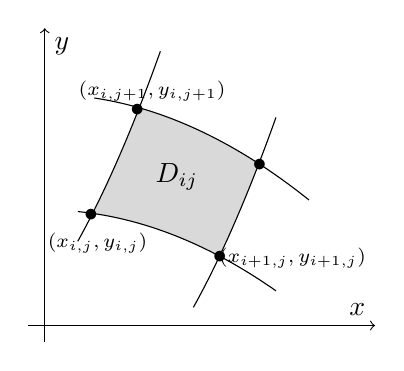
\begin{tikzpicture}[baseline]
\begin{axis}[
axis lines = middle,
unit vector ratio*=1 1 1,
scale=0.7, xmin=-0.1, xmax=2.0, ymin=-0.1, ymax=1.8,
%grid = major,
xtick={0},
ytick={0},
xticklabels = {},
yticklabels = {},
xlabel=$x$,
ylabel=$y$,
axis line style = {->},
]
\addplot[name path=up1,samples=100,domain=0.2:0.7]{(x+0.7)^2-0.3};
\addplot[name path=up2,samples=100,domain=0.3:1.6]{1.4-1/4*x^2};
\addplot[name path=below1,samples=100,domain=0.2:1.4]{0.7-1/4*x^2};
\addplot[name path=below2,samples=100,domain=0.9:1.4]{x^2-0.7};
\addplot[gray!30]fill between[of=up2 and below1,soft clip={domain=0.3:1.3}];
\addplot[white]fill between[of=up1 and up2];
\addplot[white]fill between[of=below2 and below1];
\node at (axis cs:0.8,0.9){$D_{ij}$};
\node at (axis cs:0.28,0.67){$\bullet$};
\node at (axis cs:0.56,1.3){$\bullet$};
\node at (axis cs:1.06,0.41){$\bullet$};
\node at (axis cs:1.3,0.97){$\bullet$};
\node at (axis cs:0.32,0.5){\scriptsize$(x_{i,j}, y_{i, j})$};
\node at (axis cs:0.65,1.42){\scriptsize$(x_{i,j+1}, y_{i, j+1})$};
\node at (axis cs:1.5,0.41){\scriptsize$(x_{i+1, j}, y_{i+1, j})$};
\end{axis}
\end{tikzpicture}

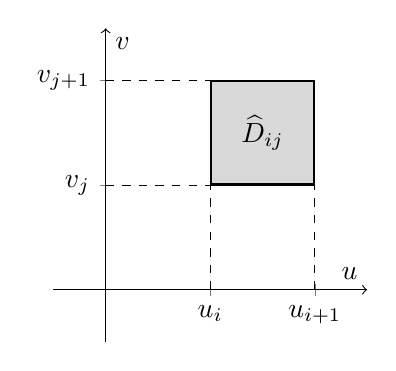
\begin{tikzpicture}[baseline]
\begin{axis}[
axis lines = middle,
unit vector ratio*=1 1 1,
scale=0.7, xmin=-0.1, xmax=0.5, ymin=-0.1, ymax=0.5,
%grid = major,
xtick={0,0.2,0.4},
ytick={0,0.2,0.4},
xticklabels = {,$u_i$,$u_{i+1}$},
yticklabels = {,$v_j$,$v_{j+1}$},
xlabel=$u$,
ylabel=$v$,
axis line style = {->},
]
    \draw[thin,dashed] (axis cs:0.2,0) -- (axis cs:0.2,0.2);
    \draw[thin,dashed] (axis cs:0.4,0) -- (axis cs:0.4,0.2);
    \draw[thin,dashed] (axis cs:0,0.2) -- (axis cs:0.2,0.2);
    \draw[thin,dashed] (axis cs:0,0.4) -- (axis cs:0.2,0.4);
    \fill[gray!30] (axis cs:0.201,0.201) rectangle (axis cs:0.399,0.399);
    \draw[thick](axis cs:0.201,0.201) rectangle (axis cs:0.399,0.399);
    \node at (axis cs:0.3,0.3){$\widehat{D}_{ij}$};
\end{axis}
\end{tikzpicture}

\end{document}